\section{Performance}
To establish the performance of the final code, a comparison is made to a baseline code in Table \ref{table:table1}, using the first day data. The baseline code, that is our first version of the solution, buses only travel, pick up passengers and drop off them. In the final version, all the improvements explained in Section \ref{sec:conceptual} are implemented.

\begin{table*}[htbp]
\centering
\begin{tabular}{ |c|c|c|  }
 \hline
  Measurement & Baseline & Final Code \\
 \hline
  Avg travel time & 150 & 72.31 \\
  Buses' expenses & 1039682 & 696162.5 \\
  Messages sent & 0 & 267  \\
  Final amount waiting & 232 & 248 \\
  Avg travel time remaining & 100 & 89.62 \\
  Final avg travel time & 156 & 75.38 \\
 \hline
\end{tabular}
\label{table:table1}
\caption{Performance results}
\end{table*}

Table \ref{table:table1} shows that there is a significant decrease in the average travelling times and in the expenses. Obviously, the number of messages increase (using the first version, no message was sent). However, the number of people waiting at the end of the simulation slightly increases in the new version.

This result highlight the advantages of an intelligent coordination and competion between buses compared to a system of buses that does not exploit these concepts.

From figure \ref{fig:pass_waiting} can be gathered that there is a peek in the number of passengers waiting during the morning rush hours. This peek lowers, when more buses are added. Thanks to the enlarged bus fleet, a smaller peek is seen during the second rush hour in the evening.

\begin{figure}[htbp]
\centering
\begin{minipage}{.48\textwidth}
  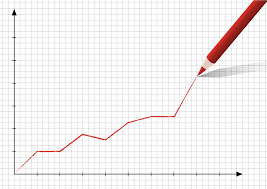
\includegraphics[width=.4\textwidth]{src/expenses.jpg}
  \caption{\label{fig:expense}Figure that displays the expenses of the buses.}
\end{minipage}%
\begin{minipage}{.48\textwidth}
  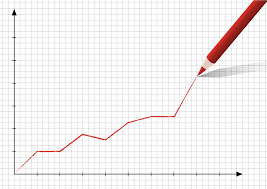
\includegraphics[width=.4\textwidth]{src/nr_messages.jpg}
  \caption{\label{fig:messages}Figure that displays the number of exchanged messages.}
\end{minipage}
\end{figure}

\begin{figure}[htbp]
\centering
\begin{minipage}{.48\textwidth}
  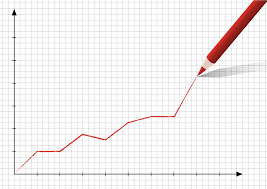
\includegraphics[width=.4\linewidth]{src/nr_pass_waiting.jpg}
  \caption{\label{fig:pass_waiting}Figure that displays the number of passengers waiting.}
\end{minipage}%
\begin{minipage}{.48\textwidth}
  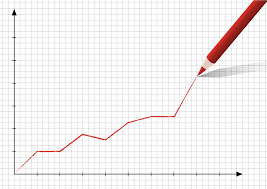
\includegraphics[width=.4\linewidth]{src/avg_tt.jpg}
  \caption{\label{fig:avg_tt}Figure that displays the average travelling time.}
\end{minipage}
\end{figure}
